\documentclass[a4paper, 11pt]{article}
\usepackage{color}
\usepackage{epic,eepic}
\usepackage{pspicture}
\usepackage{pstcol,pst-node,pst-tree,graphics}
\usepackage[dvips]{graphicx}
%\usepackage[dvips]{rotating}
\usepackage[colorlinks]{hyperref}
\usepackage[all,poly]{xy}

\DeclareGraphicsRule{.jpg}{eps}{.jpg.bb}{`jpeg2ps -r 0 -h #1}
\DeclareGraphicsRule{.gif}{eps}{.gif.bb}{`convert #1 eps2:-}
\DeclareGraphicsRule{.tif}{eps}{.tif.bb}{`tiff2ps -e -2 #1}
\DeclareGraphicsRule{.ps.bz2}{eps}{.ps.bb}{}
\DeclareGraphicsRule{.emf}{bmp}{}{}

\author{Fabrice Popineau}
\title{\colorbox{red}{\textcolor{yellow}{Windvi 0.65 Features}}}
\date{\textcolor{blue}{21/07/1998}}
\pagestyle{empty}

\def\WDVI{\textsf{Windvi}}
\newcommand{\HR}{\rule{1em}{0.4pt}}
\begin{document}
\maketitle
\tableofcontents
\newpage
\section{Introduction}
\noindent
Many of these examples are taken from the \emph{LaTeX Graphics Companion}.

\noindent First, we check the color text behavior:

\begin{flushleft}
{\color{green} green text}\\
{\color{red} red text}\\
{\color{yellow} yellow text}\\
{\color{magenta} magenta text}\\
{\color{cyan} cyan text}
\end{flushleft}
%

This is the default text.
\newpage
\section{Postscript inclusions}
Various effects:
\vspace*{2cm}\mbox{}\\
\setlength\fboxsep{0pt}
left\HR
\fbox{\includegraphics{wsample.ps}}%
\HR right
\hfill
left \HR
\fbox{\includegraphics[120,120][150,200]{wsample.ps}}%
\HR right \hfill
left \HR
\fbox{\includegraphics*[120,120][150,200]{wsample.ps}}%
\HR right
\vspace*{1cm}

\noindent
The same file, but in a rotated box:
\vspace*{1cm}

left\HR
\fbox{\rotatebox{45}{\includegraphics{wsample.ps}}}%
\HR right
\vspace*{1cm}

\noindent You can include the compressed versions too:
\vspace*{1cm}

left\HR
\fbox{\rotatebox{30}{\includegraphics{ws_gzip.ps.gz}}}%
\HR right
\hfill
left\HR
\fbox{\rotatebox{60}{\includegraphics{ws_bzip2.ps.bz2}}}%
\HR right
\vspace*{1cm}

The first one is GZip'ed, the second one is BZip2'ed.

\newpage
\section{Arbitrary Postscript code}

The following figure, Fig.~\ref{figf7}, is an example of raw
Postscript being sent to the driver.  It has been taken from the
{\em dvips} manual.

\begin{figure}[h]
  \vspace{2in}
  \vbox to 100bp{
    \special{" newpath 000 000 moveto 100 100 lineto 394 0 lineto
      closepath gsave 0.8 setgray fill grestore stroke}\vfil}
  \caption{Postscript code directly from a {\em special} command.}
  \label{figf7}
\end{figure}  

\noindent
This code lead to the previous figure:

\begin{verbatim}
  \vspace{2in}
  \vbox to 100bp{
    \special{" newpath 000 000 moveto 100 100 lineto 394 0 lineto
      closepath gsave 0.8 setgray fill grestore stroke}\vfil}
\end{verbatim}
\newpage
\section{TPIC specials}
A TPiC trial:\\
\setlength{\unitlength}{0.0125in}
\begin{picture}(444,125)(0,-10)
\thicklines
\drawline(304.318,26.338)(303.000,31.000)(301.969,26.267)
\put(311.808,31.269){\arc{17.624}{4.8481}{9.3942}}
\drawline(158.742,66.792)(161.000,63.000)(160.792,67.408)
\put(168.688,65.312){\arc{16.054}{2.8495}{7.4287}}
\drawline(143.367,53.233)(147.000,54.000)(143.433,55.033)
\put(147.250,60.750){\arc{13.509}{1.6078}{6.2462}}
\put(34,46){\oval(68,26)}
\put(163,46){\ellipse{22}{22}}
\put(231,46){\ellipse{22}{22}}
\put(299,46){\ellipse{22}{22}}
\put(366,46){\ellipse{22}{22}}
\put(433,46){\ellipse{22}{22}}
\drawline(73,46)(146,46)
\drawline(138.000,44.000)(146.000,46.000)(138.000,48.000)
\drawline(181,46)(214,46)
\drawline(206.000,44.000)(214.000,46.000)(206.000,48.000)
\drawline(247,46)(282,46)
\drawline(274.000,44.000)(282.000,46.000)(274.000,48.000)
\drawline(315,46)(349,46)
\drawline(341.000,44.000)(349.000,46.000)(341.000,48.000)
\drawline(383,46)(416,46)
\drawline(408.000,44.000)(416.000,46.000)(408.000,48.000)
\spline(294,34)
(254,4)(194,-1)(164,14)(159,29)
\drawline(163.427,22.043)(159.000,29.000)(159.632,20.778)
\spline(229,34)
(209,19)(184,19)(169,34)
\drawline(176.071,29.757)(169.000,34.000)(173.243,26.929)
\spline(221,35)
(199,29)(175,35)
\drawline(183.246,35.000)(175.000,35.000)(182.276,31.119)
\spline(354,59)
(294,79)(244,59)
\drawline(250.685,63.828)(244.000,59.000)(252.171,60.114)
\spline(359,64)
(318,92)(224,84)(179,55)
\drawline(184.641,61.015)(179.000,55.000)(186.808,57.652)
\put(390,52){\makebox(0,0)[lb]{\raisebox{0pt}[0pt][0pt]{\Large C}}}
\put(323,50){\makebox(0,0)[lb]{\raisebox{0pt}[0pt][0pt]{\Large B}}}
\put(298,94){\makebox(0,0)[lb]{\raisebox{0pt}[0pt][0pt]{\Large B}}}
\put(270,74){\makebox(0,0)[lb]{\raisebox{0pt}[0pt][0pt]{\Large A}}}
\put(321,16){\makebox(0,0)[lb]{\raisebox{0pt}[0pt][0pt]{\Large A}}}
\put(260,18){\makebox(0,0)[lb]{\raisebox{0pt}[0pt][0pt]{\Large C}}}
\put(258,51){\makebox(0,0)[lb]{\raisebox{0pt}[0pt][0pt]{\Large A}}}
\put(221,16){\makebox(0,0)[lb]{\raisebox{0pt}[0pt][0pt]{\Large C}}}
\put(196,35){\makebox(0,0)[lb]{\raisebox{0pt}[0pt][0pt]{\Large B}}}
\put(192,50){\makebox(0,0)[lb]{\raisebox{0pt}[0pt][0pt]{\Large A}}}
\put(167,77){\makebox(0,0)[lb]{\raisebox{0pt}[0pt][0pt]{\Large C}}}
\put(129,64){\makebox(0,0)[lb]{\raisebox{0pt}[0pt][0pt]{\Large B}}}
\put(19,42){\makebox(0,0)[lb]{\raisebox{0pt}[0pt][0pt]{\Large Start}}}
\put(162,42){\makebox(0,0)[lb]{\raisebox{0pt}[0pt][0pt]{\Large 1}}}
\put(228,42){\makebox(0,0)[lb]{\raisebox{0pt}[0pt][0pt]{\Large 2}}}
\put(298,42){\makebox(0,0)[lb]{\raisebox{0pt}[0pt][0pt]{\Large 3}}}
\put(363,42){\makebox(0,0)[lb]{\raisebox{0pt}[0pt][0pt]{\Large 4}}}
\put(432,42){\makebox(0,0)[lb]{\raisebox{0pt}[0pt][0pt]{\Large *}}}
\end{picture}

End of TPic test.

\noindent
And the \texttt{pspicture} environment:
% pspicture
\setlength{\unitlength}{1mm}
\begin{picture}(50,40)
\put(15,20){\circle{20}}
\put(40,20){%
\scalebox{1}[2]{\circle{20}}}
\put(40,20){%
\scalebox{1}[.5]{\circle*{20}}}
\end{picture}\qquad

\newpage
\section{Transformations}
\noindent
Here the text should be rotated, but given this is text, and that this
material is not processed by ghostscript, the text is not rotated.

However, under Windows NT, there is an opportunity to render this and
this is done now. \textcolor{red}{So only NT users will see the actual 
  text. }

\def\foo{\parbox{2cm}{\Huge A}}

\foo \hfill \rotatebox{30}{\foo} \rotatebox{0}{} \hfill \rotatebox{60}{\foo} \hfill
\rotatebox{90}{\foo} \hfill \rotatebox{180}{\foo}
\vspace*{2cm}\mbox{}\\
\fbox{\resizebox{5cm}{20mm}{%
    \rotatebox{45}{\parbox{3cm}%
{\raggedright
TUG96 in Russia   TUG96 in Russia
TUG96 in Russia   TUG96 in Russia
TUG96 in Russia}}}}

And with tables~:\\
\rotatebox{90}{%
  \Large
  \begin{tabular}[ht]{|l|c|r|}
    \hline 
    1 & 2 & 3 \\
    \hline
    a & b & c \\
    \hline
  \end{tabular}
}
\newpage
\section{The world of color}

\begin{enumerate}
\item \textcolor[cmyk]{0,1,0,0}{magenta cmyk} black
\item \color[gray]{0.5}
  \textcolor{blue}{predefined blue}
  gray text
\end{enumerate}

\noindent
\fcolorbox{red}{blue}{Black text, blue background, red frame}\\
\fcolorbox{red}{blue}{\color{white}White text, blue background, red
  frame}\\
\fcolorbox{red}{blue}{\color{green}Green text, blue background, red
  frame}

\setlength{\fboxrule}{6pt}
\setlength{\fboxsep}{10pt}
\colorbox{yellow}{Fun with color}\qquad
\fcolorbox{red}{yellow}{Fun with color}
\par\bigskip\par
\setlength{\fboxrule}{1pt}%
\colorbox{green}{Fun with color}\qquad
\fcolorbox{red}{green}{Fun with color}

\newpage
\section{The XY-Pic package}
\[
\begin{xy}/r9mm/:
  (0,0),{\xypolygon6{%
      ~:{(1,-.1):(0,.33)::}~<{-}}}
  ,(0,2),{\xypolygon6{%
      ~:{(1,-.2):(0,.5)::}~<{-}}}
  ,(2.5,0),{\xypolygon6{%
      ~:{(1,.2):(0,-.3)::}~<{-}}}
  ,(2.5,2),{\xypolygon6{%
      ~:{(1,.3):(0,-.6)::}~<{-}}}
  ,(5,0)="O", +(-.5,3)="T","O"
  ,{\xypolygon6{~:{(1,0.2):(0,.4)::}%
      ~<>{;"T"**@{-}}}}
\end{xy}
\]

\newpage
\section{The PSTricks package}

\psset{nodesep=2pt}
\newcommand{\XX}[2]{%
\TR{\ensuremath{#1_{\mbox{#2}}}}%
}
\pstree[xbbr=1.5cm]{\XX{R}{AMSU}}
{
\XX{S}{RawData}
\pstree{\XX{S}{combine}
  \trput{\ensuremath{\oplus}}
\tlput{\ensuremath{\oplus}}}
{
\psset{linestyle=dashed}
\XX{R}{Modes}
\XX{R}{Normal}
\XX{R}{Vertical}
\XX{R}{Latched}
\XX{R}{Tripped}
\XX{R}{Other}
}
\XX{S}{GenerateData}
}

\newpage
\noindent
This is the same tree, but rotated. Only NT users will see the glyphs
at the right place. Win9x will see the Postscript code at the right
place, but the glyphs displaced:

\rotatebox{90}{
\psset{nodesep=2pt}
\renewcommand{\XX}[2]{%
\TR{\ensuremath{#1_{\mbox{#2}}}}%
}
\pstree[xbbr=1.5cm]{\XX{R}{AMSU}}
{
\XX{S}{RawData}
\pstree{\XX{S}{combine}
  \trput{\ensuremath{\oplus}}
\tlput{\ensuremath{\oplus}}}
{
\psset{linestyle=dashed}
\XX{R}{Modes}
\XX{R}{Normal}
\XX{R}{Vertical}
\XX{R}{Latched}
\XX{R}{Tripped}
\XX{R}{Other}
}
\XX{S}{GenerateData}
}
}
\newpage
\section{Is color correctly handled ?}
\vfill

Something that is higly desirable : being able to jump to \emph{any}
page, and be placed in the correct color stack state. This is possible 
because \WDVI{} does pre-scanning of all specials.

What will happen if we {\color{blue} break some \newpage page across
  color text ?} Will we get the expected result ?

\newpage
\section{Background color for the whole page}
\pagecolor{yellow}

Test of the background for the {\color{red} windvi program}.

\newpage

Is the background restored to white ?

I hope not ! Because the \verb+\pagecolor{}+ command is sticky through
out the document.

\newpage
\section{External commands and inclusions}
\pagecolor{white}

\noindent
This is an inclusion of a \texttt{.jpg} image thanks to
\texttt{jpeg2ps.exe}.

Beware ! By default, it is forbidden to call external programs. You
need to check the `allowShell' option in the menus `View', `Options'
and next `DVI File Configuration'. Only then \windvi will be able to
display the next picture.

\begin{figure}[ht]
  \centering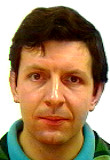
\includegraphics[width=4cm]{fab.jpg}
  \caption{The author.}
\end{figure}

\noindent Oh ! By the way : that's me. This was the easiest jpeg picture to
find.

\noindent
Now trying \texttt{.bmp} files:
\begin{figure}[ht]
  \centering\includegraphics[width=6cm,height=6cm]{coffee_bean.bmp}
  \caption{Some \texttt{bmp} file.}
\end{figure}

\newpage
\noindent
And Windows Enhanced Metafiles:
\begin{figure}[ht]
  \centering\includegraphics[width=79.34mm,height=40mm]{world.emf}
  \caption{Some \texttt{emf} file.}
\end{figure}

\end{document}
%%% Local Variables: 
%%% mode: latex
%%% TeX-master: t
%%% End: 

\end{document}

%%% Local Variables: 
%%% mode: latex
%%% TeX-master: t
%%% End: 
